\documentclass[a4paper, 14pt]{article}
\usepackage[utf8]{inputenc}
\usepackage{amsmath,amsfonts,amssymb,amsthm,mathtools} % AMS
\usepackage{wrapfig,lipsum, cleveref}
\usepackage{icomma} 
\usepackage{color}
\usepackage{geometry} 
\usepackage{longtable}
\usepackage{booktabs}

\linespread{1.5}

\geometry{top=25mm}
\geometry{bottom=35mm}
\geometry{left=35mm}
\geometry{right=20mm}


%% Номера формул
%\mathtoolsset{showonlyrefs=true} % Показывать номера только у тех формул, на которые есть \eqref{} в тексте.

%% Шрифты
\usepackage{euscript}	 % Шрифт Евклид
\usepackage{mathrsfs} % Красивый матшрифт

%% Свои команды
\DeclareMathOperator{\sgn}{\mathop{sgn}}

%% Перенос знаков в формулах (по Львовскому)
\newcommand*{\hm}[1]{#1\nobreak\discretionary{}
{\hbox{$\mathsurround=0pt #1$}}{}}


\title{Вариация алгоритма кросс-валидации со взвешиванием наблюдений}
\usepackage{cmap}					% поиск в PDF
\usepackage[T2A]{fontenc}			% кодировка
\usepackage[utf8]{inputenc}			% кодировка исходного текста
\usepackage[english,russian]{babel}	% локализация и переносы
\usepackage{graphicx}
\graphicspath{{pictures/}}
\DeclareGraphicsExtensions{.pdf,.png,.jpg}
\author{Гармидер Петр}
\date{\today}
\begin{document}


\thispagestyle{empty}
\begin{center}
	\textbf{ПРАВИТЕЛЬСТВО РОССИЙСКОЙ ФЕДЕРАЦИИ}\\
	\vspace{2ex}
	\textbf{Федеральное государственное автономное\\ образовательное учреждение высшего образования}
	
	\vspace{2ex}
	
	\textbf{Национальный исследовательский университет \\ <<Высшая школа экономики>>}
	
	\vspace{8ex}
	\begin{flushright}
		Факультет экономических наук\\
		Образовательная программа <<Экономика>>
	\end{flushright}
\end{center}
\vspace{9ex}

\begin{center}
	{\textbf{КУРСОВАЯ РАБОТА
	}}
	\vspace{1ex}
	
	На тему <<Вариация алгоритма кросс-валидации со взвешиванием наблюдений>>
\end{center}
\vspace{1ex}
\begin{flushright}
	\noindent
	Студент группы БЭК161\\Гармидер Петр Александрович\\
	\vspace{13ex}
	Научный руководитель:\\
	Борис Демешев
	
\end{flushright}	

\vfill

\begin{center}
	Москва 2019
	
\end{center}
\newpage

\tableofcontents

\newpage

\section{Введение}
\subsection{Параметры и гиперпараметры модели}
Большая часть популярных моделей имеют множество параметров и гиперпараметров однозначно выделяющие модель из множества всех алгоритмов. Гиперпараметры модели --- параметры, вводимые пользователем вручную, которые в большинстве случаев не меняются в ходе обучения\footnote{Однако такая практика также используется, например, изменение гиперпараметра  learning rate в ходе алгоритма градиентного спуска (см. \cite{zeiler2012adadelta})}. Параметры модели --- параметры, которые не вводятся пользователем вручную, а есть результат оптимизации функции потерь. Их конечное значения становится известно после завершения процесса обучения. Параметры модели связывают имеющиеся у исследователя данные и выбранный алгоритм для обучения. 

Рассмотрим пример. Пусть имеем обучающую выборку $D = \left\{x_i, y_i\right\}$ и тестовую выборку $d = \left\{x_i, y_i\right\}$, где $x_i$, $y_i$ $\in R$, $\left|D\right| = N$ и $\left|d\right| = n$. Будем оценивать $y_i$ используя $L_2$ - регуляризатор или Ridge-regression (см. \cite{hoerl1970ridge}). Имеем безусловной задачу оптимизации:


\begin{equation} \label{ridge} %% Invalid referencing
\sum_{i=1}^{N} (y_i - \hat{\beta_0} - \hat{\beta_1} x_i)^2 + \lambda \hat{\beta_1^2} \rightarrow \underset{\hat{\beta_0}, \hat{\beta_1}}{min}
\end{equation} 

В \eqref{ridge} существуют два параметра для оптимизации $\hat{\beta_0} \text{ и } \hat{\beta_1}$, а также один гиперпараметр $\lambda$, который является константой в рассматриваемой задаче. Коэффициенты регрессии находятся из задачи минимизации при заданном уровне $\lambda$, в то время, как степень регуляризации $\lambda$ задается исследователем. В конечно счете исследователь заинтересован в создании модели, которая имеет высокое качество на тестовой выборке $d$, что не участвовала в процессе обучения. Качество работы модели на выборке $d$ очевидно зависит от выбранного исследователем $\lambda$. Поэтому, выбор оптимального значения для гиперпараметров является также важной задачи для получения лучшей модели.

Гиперпараметрами модели также могут быть: метод обработки пропусков в данных, количество слоев в нейронной сети, выбранные функции активации, уровень Dropout, скорость обучения и другие. 

Влияние гиперпараметров на качество работы модели делает их правильный выбор отдельной задачей. Оптимальный алгоритм подбора гиперпараметров уникален для каждой конкретной задачи. Качество работы модели в целом принято оценивать на выборках не участвовавших в обучении, но для которых известно истинной значение зависимой переменной. 

\subsection{Типы кросс-валидации}
Кросс-валидация --- техника валидации модели для оценки качества её работы и установления факта обобщающей способности. Метод CV позволяет понять, выучила ли модель зависимость между рассматриваемыми переменными или же алгоритм переобучился и хорошо предсказывает лишь данные имеющиеся в обучающей выборке\footnote{В английской литературе данную ситуацию называют 	overfitting}. Как правило, кросс-валидационной проверке подвергаются модели, которые направлены на точность предсказаний, оставляя за бортом вопрос интерпретации полученных результатов.  

\noindent Разберем некоторые варианты алгоритма кросс-валидации:

\noindent Пусть имеем: $X$ --- множество признаков, описывающих объекты; $Y$ --- множество зависимых переменных; $D^l = \left\{x_i, y_i\right\}$ --- наблюдаемая выборка , где $x_i \in X$, $y_i \in Y$, $l$ --- размер выборки; $Q : (A \times (X \times Y ) )  \rightarrow R$ --- функция потерь; $A$ --- модель; $\mu : (X \times Y) \rightarrow A$ --- алгоритм обучения \cite{ifmocv}.

\label{CV_methods}
\begin{itemize}
	\item Валидация на отложенных данных (Hold-out)
	
	Исследователь выбирает число $t$ --- количество объектов из множества $D$, которые будут использованы для обучения модели. Соответственно, оставшая часть объектов $l - t$ используется для проверки качетсва работы модели. Итого, получаются две выборки $Train^t \text{ и } Test^{l-t}$ такие, что $Tr^t \cup Tt^{l-t} = D^l$. Решается задача:
	
	\[HOCV(\mu, Tr^t, Tt^{l-t}) = Q(\mu (Tr^t), Tt^{l-t}) \rightarrow \underset{\mu}{min} \] 
	
	\begin{figure}[h]
		\center{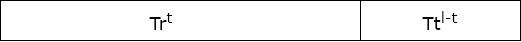
\includegraphics[scale=0.55]{img/Hold-out}}
		\label{ris: ho}
		\caption{Иллюстрация валидации на отложенных данных}
	\end{figure}
	
	
	Метод Hold-out CV обычно используется в том случае, если исследователь обладает большой обучающей выборкой, т.к данный способ не требует больших вычислительных мощностей. Итоговое качество $Q$ также зависит от разбиения обучающей выборки, что является главным недостатком метода. 
	
	\item K-fold кросс-валидация 
	
	Исходная выборка $D$ разбивается случайным образом на $K$ непересекающихся, примерно равных по мощности множеств: $D_1$, $D_2$, $\dots$ $D_k$; $\left|D_i\right| \approx \frac{l}{k}$. После чего, для каждого из получившихся множеств проводится процедура hold-out CV; результаты всех процедур усредняются. Решается задача:
	
	\[KFCV(\mu, D, K) = \frac{1}{K} \sum_{i=1}^{K} OFCV(\mu(D \textbackslash D_i), D_i) \rightarrow \underset{\mu}{min} \]
	
	\begin{figure}[h]
		\center{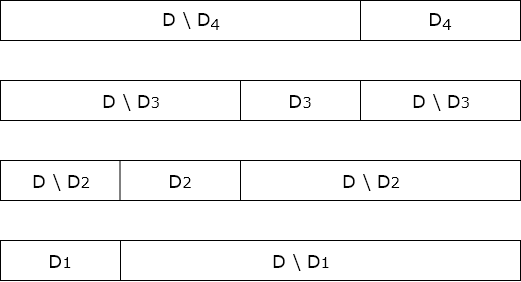
\includegraphics[scale=0.55]{img/K_CV}}
		\label{ris: kfold}
		\caption{Иллюстрация K-fold кросс-валидации при $K=4$}
	\end{figure}
	
	Метод K-fold CV решает проблему высокой зависимости получаемого результата от разбиения, однако является весьма затратным с точки зрения вычислительных мощностей. Обычно используется в тех случаях, когда размеры выборки и модель позволяют быстро проводить процедуру обучения. Число K выбирается исследователем на своё усмотрение. Заметим, что при $t = \frac{l}{2}$ Hold-out CV $ \equiv $ two-fold CV.
	
	\item Leave-one-out кросс-валидация
	
	Частный случай K-fold кросс-валидации, при $K=l$. Исходное множество $D$ разбивается на $l$ подмножеств: $D_1$, $D_2$, $\dots$ $D_l$; $\left|D_i\right| = 1$. После чего проводится стандартная K-fold кросс-валидация. LOO CV подвергается критике; в некоторых исследованиях говорится, что данный метод плохо оценивает предсказательную силу модели \cite{efron1986biased}. Кроме того, данный метод требует высоких вычислительных мощностей, т.к потребуется $l$ раз обучать модель.
	
	\item Полная кросс-валидация (Complete)
	
	Исследователь выбирает число $t$, после чего изначальная выборка $D^l$ разбивается всеми возможными способами на выборки $Tr^l$ и $Tt^{l-t}$. Заметим, что силов возможных разбиений для заданного t равно $C_l^{l-t}$. Таким образом, исследователь решает задачу:
	
	\[CCV(D, t) = \frac{1}{C_l^{l-t}} \sum_{D^l = Tr^l \cup Tt^{l-t}} Q(\mu (Tr^t), Tt^{l-t}) \rightarrow \underset{\mu}{min} \]
	
	Даже при достаточно небольших значениях t, данный метод проверки работоспособности модели используется крайне редко в силу его вычислительной сложности.
	
	\item Случайные разбиения (Random sampling)
	
	Выборка разбивается в случайной пропорции, после чего для получившегося разбиения проводится hold-out CV. Данная процедура повторяется несколько раз; результаты усредняются. 
	
	
	\item M $\times$ K-fold кросс-валидация
	
	K-fold кросс-валидация проводится M раз; результаты М валидаций усредняются. Итого: 
	
	\[MKFCV(\mu, D, K, M) = \frac{1}{M} \sum_{i=1}^{M} KFCV(\mu, D, K) \rightarrow \underset{\mu}{min}  \]
	
	Метод допустим к использованию при небольшой выборке и алгоритме, который способен обучаться $M \times K$ раз за разумное время.
\end{itemize}

Одной из причин использования кросс-валидации является подбор гиперпараметров. Допустим исследователь решает задачу по выбору оптимального параметра $\lambda$ для $L_2$ - регуляризатора на странице \pageref{ridge}. Если не проводить кросс-валидацию, то лучшее качество на выборке $D$ даст модель с $\lambda = 0$, т.к в этом случае на коэффициенты регрессии не накладываются никакие ограничения, а поэтому они сойдутся к решению, которое минимизирует среднеквадратичную ошибку на выборке $D$. Однако, получаемое качество работы модели на обучающей выборке не отображает реальную картину. Исследователь, в конечном счете, заинтересован создать модель, которая будет иметь высокое качество на объектах не входящих в обучающую выборку. Для этого, есть смысл проверять качество работы модели используя один из перечисленных методов кросс-валидации. В этом случае, оптимальное значение $\lambda$ скорее всего окажется больше нуля.

\subsection{Кросс-валидация для временных рядов}

Временной ряд --- наблюдаемая выборка данных, объекты которой представлены во временном порядке. В большинстве случаев, временной ряд представлен точками, которые одинаково отдалены друг от друга во временной шкале. Анализ временных рядов значимо отличается от подходов работы с простой выборкой данных:  учитывается зависимость точек от времени, а также взаимосвязь текущего значения параметра с лагированными. Примерами временных рядов являются: курс доллар к евро, реальный уровень ВВП США, ключевая ставка ЦБ РФ, последовательность кадров в видеоролике\footnote{Объектами в таком случае являются трехмерные матрицы, хранящие в себе значения, характеризующее интенсивность RGB каналов} и так далее. В данной работе фокус будет сделан на одномерных временных рядах, прогноз для которых будет иметь вид некоторой функции от прошлых значений. 

Как и раньше, задача построения моделей для прогнозирования временных рядов включает в себя стадию подбора оптимальных гиперпараметров модели. Однако, по очевидным причинам большинство методов кросс-валидации из секции \ref{CV_methods} не подходят для случая, когда объектом исследования является временной ряд. Непрактично оценивать модель на случайно выбранных данных, которые с большой долей вероятности потеряют временную структуру при разбиениях. 

Очевидным решением в таком случае является разбиение исходной выборки на две части: обучающую и валидационную --- с сохранением временной структуры. После чего на последней измерять качество работы модели. Тем не менее, проблема высокой зависимости результата от разбиения становится вновь актуальной. Возможно, исследователь столкнется с ситуацией, когда качественная модель плохо справляется лишь с отведенным для валидации блоком данных, но будет давать прогнозы с высокой точностью в долгосрочной перспективе. 

Решением данной проблемы является адаптированный алгоритм K-fold кросс-валидации для временных рядов (K-fold TSCV):

\noindent Пусть $TS = \left\{y_t\right\}$ --- наблюдаемая выборка временного ряда, где $\left|TS\right| = T$, $t = 1, 2, \dots,  T$; $\lambda \in \Lambda$, где $\Lambda$ --- множество всех доступных гиперпараметров для модели $\mu$. Исследователь выбирает число K, после чего TS делится на K блоков: $TS_1$, $TS_2$, \dots $TS_K$; $\left|TS_i\right| \approx \frac{T}{K}$; 
$TS_i = \left\{y_j, y_{j+1}, y_{j+2}  \dots \right\}$. Затем, выбранная модель $\mu$ обучается $K-1$ раз следующим образом: обучение проходит на $TS_1$ --- качество проверятся на $TS_2$, обучение проходит на $TS_1 \cup TS_2$ --- качество проверяется на $TS_3$ и так далее. Для подбора оптимального гиперпараметра $\lambda$ для модели $\mu$ исследователь решает задачу:

\begin{equation}\label{TSCV}
TSCV_K = \frac{1}{K-1} \sum_{i=1}^{K-1} Q(\mu(TS_1 \cup \dots \cup TS_i, \lambda), TS_{i+1}) \rightarrow \underset{\lambda \in \Lambda}{min}
\end{equation}

\begin{figure}[h]\label{ris: tscv}
	\center{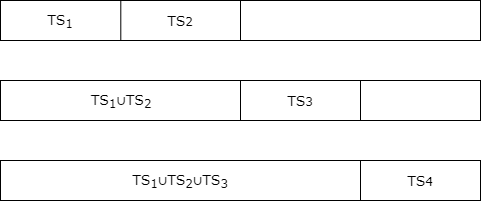
\includegraphics[scale=0.6]{img/tscv}}
	\caption{Иллюстрация K-fold кросс-валидации для временных рядов при $K=4$}
\end{figure}

Описанный подход также не является идеальным решением и плохо работает в случаях, когда наблюдений не так много, а следовательно, алгоритму на первых итерациях предстоит обучаться на малом количестве наблюдений и измерять качество на такой же по количеству выборке. Очевидно, что в таких ситуациях модель покажет низкое качество, но это не значит, что она не применима для качественного прогнозирования рассматриваемого ряда.

\newpage

\section{Взвешенная кросс-валидация для временных рядов}
\subsection{Мотивация}

Зависимость временного ряда во времени делает его весьма интересным объектом для изучения. Как правило, рассматриваемые в прикладных задачах ряды являются объектами человеческой деятельность: продажи товаров, количество новых клиентов, --- что по определению делает такие ряды подверженными внешним шокам. Хотелось бы подобрать такой алгоритм, который устойчив к данным изменениям и способен хорошо предсказывать будущие значения по всей имеющейся информации на сегодняшний день. В некоторой степени данную задачу может разрешить алгоритм ETS с аккуратно подобранными гипермараметрами. Ввиду особенностей своей работы ETS позволяет моделировать, например, изменение долгосрочного уровня в ответ на произошедшие в прошлом шоки. Однако, дабы такая модель была решением задачи поиска оптимального алгоритма на кросс-валидации для временных рядов, ETS также должна хорошо предсказывать прошлые данные в то время, когда исследователя, как правило, интересуют актуальные наблюдения. Данные рассуждения наталкивают на идею модификации алгоритма кросс-валидации для устранения упомянутой проблемы.

\begin{figure}[h]\label{ris: gofo}
	\center{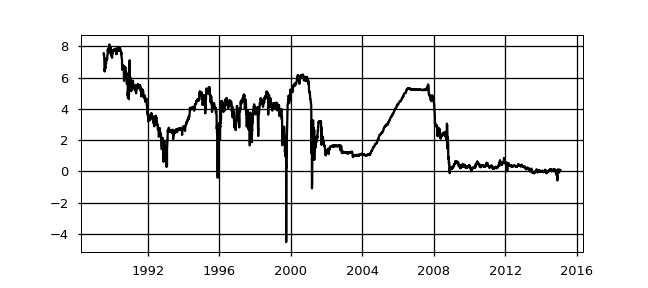
\includegraphics[scale=0.65]{img/gofo-1m}}
	\caption{Месячный форвардный курс золота (GOFO), в процентах \cite{quandlGOFO}}
\end{figure}

Чтобы показать, что ситуация описанная выше не является теоретизированной,  рассмотрим рис. 4. %ref isn't working for some reasons%
На данном графике изображен месячный форвардный курс золота в процентах от текущей стоимости за период с 1990 по начало 2015 года. Довольно очевидно, учитывая имеющиеся данные за последние 8 лет, что сильным и, возможно, наилучшим прогнозом для рассматриваемого ряда на ближайшее время будет векторов скаляров в окрестности нуля. Однако, маловероятно, что такая модель будет отобрана на кросс-валидации, учитывая поведение ряда до 2009 года. Видно, что ряд имел участки, где присутствуют: линейно-возрастающий тренд; линейно-убывающим тренд; ярковыраженная сезонность и другие особенности, которые не свойственны актуальным наблюдениям. Некоторый класс моделей справляются и с такими особенностями ряда. Однако, хотелось бы адаптировать процесс кросс-валидации так, чтобы практически любая модель имела устойчивость к изменчивости характеристик временного ряда, при процессе подбора гиперпараметров 

\subsection{Описание алгоритма}

Основная идея за предлагаемым алгоритмом заключается в вере о том, что модель, которая качественно предсказывает последние наблюдения лучше той, что хорошо работает лишь на давних участках данных. Действительно, часто исследователя вовсе не волнует ситуация, когда модель совершенно не справляется с давними участками, если алгоритм показывает высокое качество на актуальных. Данный факт обуславливается тем, что временные ряды зачастую используются для принятия решений в данный момент времени, основываясь на мнении о том, что будет завтра. Поэтому для пользователя важно иметь высокое качество в прогнозах именно на завтра\footnote{Существуют задачи, целью которых является качественные прогнозирование прошлых периодов. Например, восстановление пропущенных данных о темпе роста ВВП нынешней РФ в период советской власти}. 

Отсюда вытекает обобщение существующего алгоритма кросс-валидации. Предлагается учитывать качество работы модели на недавних участках с большим весом, а качество работы модели в далеком прошлом с меньшим или не учитывать вовсе. Формально задача сводится к следующей:

\noindent Пусть $TS = \left\{y_t\right\}$ --- наблюдаемая выборка временного ряда, где $\left|TS\right| = T$, $t = 1, 2, \dots,  T$; $n(y)$ --- номер наблюдения $y$: $n(y_i) = i$; $Q(a,b)$ --- некоторая функция, измеряющая различие $a$ и $b$; $\mu (\lambda)$ --- алгоритм прогнозирования; $\lambda \in \Lambda$, где $\Lambda$ --- множество всех доступных гиперпараметров для $\mu$. Проводим стандартную K-fold кросс-валидацию для временных рядов \eqref{TSCV}, сохраняя при этом предсказания модели для каждого объекта из отложенных выборок: $TS_2$, $TS_3$, \dots $TS_K$. Итого, для алгоритма $\mu(\lambda)$ имеем $\approx \frac{(K-1)T}{K}$ предсказаний для объектов на отложенных выборках\footnote{$TS_1$ требуется для изначального обучения модели на первой итерации \eqref{TSCV}}. Данные предсказания составляют множество $V(\mu(\lambda))$. Тогда подбор оптимального гиперпараметра $\lambda$ для модели $\mu$ сводится к следующей задаче минимизации:

\begin{equation}\label{WTSCV}
\sum_{\hat y \in V(\mu(\lambda))} Q(\hat y, y) \gamma^{T - n(y)} \rightarrow \underset{\lambda \in \Lambda}{min}
\end{equation}
где $\gamma \in \left[0, 1\right]$ --- константа отражающая степень важности предсказаний на более актуальных данных временного ряда: $\gamma = 1$ $\Leftrightarrow$ стандартный алгоритм K-fold TSCV \eqref{TSCV} --- $\gamma = 0$ $\Leftrightarrow$ важно качество предсказания алгоритма только на последнем имеющимся наблюдении $y: n(y) = T$. Таким образом, константа $\gamma$ позволяет моделям с лучшим качеством работы на актуальных данных выигрывать у моделей, показывающих себя средне на всей выборке. Таким образом, получаем обобщенную версию метода \eqref{TSCV} --- взвешенную K-fold кросс-валидацию для временных рядов (K-fold WTSCV). Схожая по идее методика уже была использована в \cite{donate2013time}, однако, авторы взвешивали качество работы не по наблюдениям, а на всей отложенной выборке, т.е. множитель $\gamma$ добавлялся в базовую модель кросс-валидации \eqref{TSCV} для всей валидационной выборки на каждой из итераций.

Очевидным недостатком данного подхода является необходимость выбора оптимальной константы $\gamma$, что делает этот метод неприменимым в случае небольшого размера наблюдаемой выборки $TS$. Остается проверить целесообразность применения данного подхода. 


\subsection{Метод тестирование подхода}

Проведем эксперимент на 1000 случайных рядах с месячной периодичностью, выбранных из набора M4 competition \cite{m4}.


\noindent Заведем переменную $S = 0$. Для каждого ряда $TS_i$ проведем следующую процедуру:

\begin{itemize} \label{desc: WTSCV}
	\item Исследуемый ряд $TS_i$ с сохранением временной структуры разбиваем в пропорции 5 к 1 на два ряда: $TS_{iCV}$ и $TS_{i\gamma}$.
	\item На данных $TS_{iCV}$ для каждого $\gamma \in \left[0, 0.99\right]$ с шагом 0.02 решаем задачу \eqref{WTSCV} при условии $\lambda \in \tilde{\Lambda} : \tilde{\Lambda} \subseteq \Lambda$. Имеем множество решений $\L = \left\{ \lambda_{\bar{\gamma}} \right\}$, где $\lambda_{\bar{\gamma}}$ --- решение задачи оптимизации при $\gamma = \bar{\gamma}$.
	\item После чего на участке $TS_{i\gamma}$ проверяем качество работы $q_{\bar{\gamma}}$ полученных моделей $\mu(\lambda_{\bar{\gamma}}) : \forall \lambda_{\bar{\gamma}} \in \L$. Записываем полученные результаты в множество $Q = \left\{q_{\bar{\gamma}}\right\}$.
	\item Находим $\gamma^* : q_{\gamma^*} \leq  q_{{\tilde{\gamma}}},   \forall q_{{\tilde{\gamma}}} \in Q$.
	\item На данных $TS_{iCV}$ подбираем оптимальный гиперпараметр $\lambda_{1}$ согласно стандартной процедуре \eqref{TSCV}. Сохраняем качество работы $\mu(\lambda_{1})$ на участке $TS_{i\gamma}$ в переменную $q_1$ .
	\item Обновим $S := S + \left[q_{\gamma^*} < q_1 \right]$
\end{itemize}

Объектом для интереса служит отношение $\frac{S}{1000}$ (Improvement rate) --- доля случаев, когда модель выбранная с помощью взвешенной кросс-валидации показала строго лучший прогноз на участке $TS_{i\gamma}$, чем модель отобранная на стандартной кросс-валидации.

Будем проверять модель на трёх разных алгоритмах используемых для прогнозирования временных рядов: Random Forest, SARIMA и Exponential Smoothing. У каждого алгоритма будем подбирать свой гиперпараметр. У RandomForest в качестве гиперпараметра будем перебирать $p$ --- кол-во лагов используемых для прогноза в периоде $t$, т.е. прогноз алгоритма будет иметь вид: 
\[ \hat y_t = RF(y_{t-1}, \dots , y_{t-p} ) \]

У SARIMA модели будем перебирать параметры p, d и q. Для ускорения эксперимента зафиксируем P, D и Q сезонные на уровне (0, 0, 0). Поскольку эксперимент будет проводиться на временных рядах с месячной периодичностью, то можем смело установить параметр сезонности $S = 12$.

Для модели ES будем перебирать всего два параметра для тренда и сезонности: аддитивность и мультипликативность. Как увидим далее, даже при столь жестких ограничениях на множество допустимых гиперпараметров модель взвешенной кросс-валидации даст заметное улучшение в сравнению со стандартным подходом. 

\noindent Для измерения качества работы моделей будем использовать метрику $MAPE$ (Mean Absolute Percentage Error) --- средняя абсолютная ошибка в процентах. 
	\[MAPE = \dfrac{1}{n} \sum_{i=1}^{n} \left|	 \dfrac{y_i - \hat y_i}{y_i} \right| 100 \% \] 
	
\section{Заключение}

В таблице 1 приведены результаты вышеописанного эксперимента. Видим, что модифицированная версия алгоритма улучшает качество дальнейших предсказаний в среднем на 33 \%. Иначе говоря, в одном из трех случаев подбор оптимального $\gamma$ дает улучшение прогнозов на актуальных участках. Это говорит о том, что для получения более точных прогнозов имеет пожертвовать частью данных для подбора оптимального параметра $\gamma$, который позволит выбрать модель, которая хорошо будет предсказывать данные будущих периодов.

\begin{table}[h] \label{res} %not working for some reasons%
	\centering
	\begin{tabular}{@{}crlll@{}}
		\toprule
		Модель                         & \multicolumn{4}{c}{Improvement rate} \\ \midrule
		\textbf{Radnom Forest}         & \multicolumn{4}{r}{0.214}                \\
		\textbf{SARIMA}                & \multicolumn{4}{r}{0.413}                \\
		\textbf{Exponential Smoothing} & \multicolumn{4}{r}{0.373}                \\ \bottomrule
	\end{tabular}
	\caption{Результаты применения Weighted Time-Series Cross-Validation}
\end{table}


Можно продолжить проверку данного подхода на других алгоритмах, однако уже видно, что даже для простых моделей взвешенный подход дает результат. 






\newpage
\bibliographystyle{utf8gost705u}  %% стилевой файл для оформления по ГОСТу
\bibliography{biblio}     %% имя библиографической базы (bib-файла) 


\end{document}
